\documentclass[]{book}
\usepackage[]{mathpazo}
\usepackage{amssymb,amsmath}
\usepackage{ifxetex,ifluatex}
\usepackage{fixltx2e} % provides \textsubscript
\ifnum 0\ifxetex 1\fi\ifluatex 1\fi=0 % if pdftex
  \usepackage[T1]{fontenc}
  \usepackage[utf8]{inputenc}
\else % if luatex or xelatex
  \ifxetex
    \usepackage{mathspec}
  \else
    \usepackage{fontspec}
  \fi
  \defaultfontfeatures{Ligatures=TeX,Scale=MatchLowercase}
\fi
% use upquote if available, for straight quotes in verbatim environments
\IfFileExists{upquote.sty}{\usepackage{upquote}}{}
% use microtype if available
\IfFileExists{microtype.sty}{%
\usepackage[]{microtype}
\UseMicrotypeSet[protrusion]{basicmath} % disable protrusion for tt fonts
}{}
\PassOptionsToPackage{hyphens}{url} % url is loaded by hyperref
\usepackage[unicode=true]{hyperref}
\PassOptionsToPackage{usenames,dvipsnames}{color} % color is loaded by hyperref
\hypersetup{
            pdftitle={Biology 3103 - Ecology Laboratory},
            pdfauthor={S Cook},
            colorlinks=true,
            linkcolor=Maroon,
            citecolor=Blue,
            urlcolor=Blue,
            breaklinks=true}
\urlstyle{same}  % don't use monospace font for urls
\usepackage{natbib}
\bibliographystyle{apalike}
\usepackage{color}
\usepackage{fancyvrb}
\newcommand{\VerbBar}{|}
\newcommand{\VERB}{\Verb[commandchars=\\\{\}]}
\DefineVerbatimEnvironment{Highlighting}{Verbatim}{commandchars=\\\{\}}
% Add ',fontsize=\small' for more characters per line
\usepackage{framed}
\definecolor{shadecolor}{RGB}{248,248,248}
\newenvironment{Shaded}{\begin{snugshade}}{\end{snugshade}}
\newcommand{\KeywordTok}[1]{\textcolor[rgb]{0.13,0.29,0.53}{\textbf{#1}}}
\newcommand{\DataTypeTok}[1]{\textcolor[rgb]{0.13,0.29,0.53}{#1}}
\newcommand{\DecValTok}[1]{\textcolor[rgb]{0.00,0.00,0.81}{#1}}
\newcommand{\BaseNTok}[1]{\textcolor[rgb]{0.00,0.00,0.81}{#1}}
\newcommand{\FloatTok}[1]{\textcolor[rgb]{0.00,0.00,0.81}{#1}}
\newcommand{\ConstantTok}[1]{\textcolor[rgb]{0.00,0.00,0.00}{#1}}
\newcommand{\CharTok}[1]{\textcolor[rgb]{0.31,0.60,0.02}{#1}}
\newcommand{\SpecialCharTok}[1]{\textcolor[rgb]{0.00,0.00,0.00}{#1}}
\newcommand{\StringTok}[1]{\textcolor[rgb]{0.31,0.60,0.02}{#1}}
\newcommand{\VerbatimStringTok}[1]{\textcolor[rgb]{0.31,0.60,0.02}{#1}}
\newcommand{\SpecialStringTok}[1]{\textcolor[rgb]{0.31,0.60,0.02}{#1}}
\newcommand{\ImportTok}[1]{#1}
\newcommand{\CommentTok}[1]{\textcolor[rgb]{0.56,0.35,0.01}{\textit{#1}}}
\newcommand{\DocumentationTok}[1]{\textcolor[rgb]{0.56,0.35,0.01}{\textbf{\textit{#1}}}}
\newcommand{\AnnotationTok}[1]{\textcolor[rgb]{0.56,0.35,0.01}{\textbf{\textit{#1}}}}
\newcommand{\CommentVarTok}[1]{\textcolor[rgb]{0.56,0.35,0.01}{\textbf{\textit{#1}}}}
\newcommand{\OtherTok}[1]{\textcolor[rgb]{0.56,0.35,0.01}{#1}}
\newcommand{\FunctionTok}[1]{\textcolor[rgb]{0.00,0.00,0.00}{#1}}
\newcommand{\VariableTok}[1]{\textcolor[rgb]{0.00,0.00,0.00}{#1}}
\newcommand{\ControlFlowTok}[1]{\textcolor[rgb]{0.13,0.29,0.53}{\textbf{#1}}}
\newcommand{\OperatorTok}[1]{\textcolor[rgb]{0.81,0.36,0.00}{\textbf{#1}}}
\newcommand{\BuiltInTok}[1]{#1}
\newcommand{\ExtensionTok}[1]{#1}
\newcommand{\PreprocessorTok}[1]{\textcolor[rgb]{0.56,0.35,0.01}{\textit{#1}}}
\newcommand{\AttributeTok}[1]{\textcolor[rgb]{0.77,0.63,0.00}{#1}}
\newcommand{\RegionMarkerTok}[1]{#1}
\newcommand{\InformationTok}[1]{\textcolor[rgb]{0.56,0.35,0.01}{\textbf{\textit{#1}}}}
\newcommand{\WarningTok}[1]{\textcolor[rgb]{0.56,0.35,0.01}{\textbf{\textit{#1}}}}
\newcommand{\AlertTok}[1]{\textcolor[rgb]{0.94,0.16,0.16}{#1}}
\newcommand{\ErrorTok}[1]{\textcolor[rgb]{0.64,0.00,0.00}{\textbf{#1}}}
\newcommand{\NormalTok}[1]{#1}
\usepackage{longtable,booktabs}
% Fix footnotes in tables (requires footnote package)
\IfFileExists{footnote.sty}{\usepackage{footnote}\makesavenoteenv{long table}}{}
\usepackage{graphicx,grffile}
\makeatletter
\def\maxwidth{\ifdim\Gin@nat@width>\linewidth\linewidth\else\Gin@nat@width\fi}
\def\maxheight{\ifdim\Gin@nat@height>\textheight\textheight\else\Gin@nat@height\fi}
\makeatother
% Scale images if necessary, so that they will not overflow the page
% margins by default, and it is still possible to overwrite the defaults
% using explicit options in \includegraphics[width, height, ...]{}
\setkeys{Gin}{width=\maxwidth,height=\maxheight,keepaspectratio}
\IfFileExists{parskip.sty}{%
\usepackage{parskip}
}{% else
\setlength{\parindent}{0pt}
\setlength{\parskip}{6pt plus 2pt minus 1pt}
}
\setlength{\emergencystretch}{3em}  % prevent overfull lines
\providecommand{\tightlist}{%
  \setlength{\itemsep}{0pt}\setlength{\parskip}{0pt}}
\setcounter{secnumdepth}{5}
% Redefines (sub)paragraphs to behave more like sections
\ifx\paragraph\undefined\else
\let\oldparagraph\paragraph
\renewcommand{\paragraph}[1]{\oldparagraph{#1}\mbox{}}
\fi
\ifx\subparagraph\undefined\else
\let\oldsubparagraph\subparagraph
\renewcommand{\subparagraph}[1]{\oldsubparagraph{#1}\mbox{}}
\fi

% set default figure placement to htbp
\makeatletter
\def\fps@figure{htbp}
\makeatother

\usepackage{booktabs}
\usepackage{longtable}
\usepackage{multicol}
\usepackage{textgreek}
\usepackage{array}
\usepackage{multirow}
\usepackage[table]{xcolor}
\usepackage{wrapfig}
\usepackage{float}
\usepackage{colortbl}
\usepackage{pdflscape}
\usepackage{tabu}
\usepackage{threeparttable}
\usepackage{threeparttablex}
\usepackage[normalem]{ulem}
\usepackage{makecell}

\usepackage[bf,singlelinecheck=off]{caption}

\usepackage{framed,color}
\definecolor{shadecolor}{RGB}{248,248,248}

\renewcommand{\textfraction}{0.05}
\renewcommand{\topfraction}{0.8}
\renewcommand{\bottomfraction}{0.8}
\renewcommand{\floatpagefraction}{0.75}

\renewenvironment{quote}{\begin{VF}}{\end{VF}}
\let\oldhref\href
\renewcommand{\href}[2]{#2\footnote{\url{#1}}}

\makeatletter
\newenvironment{kframe}{%
\medskip{}
\setlength{\fboxsep}{.8em}
 \def\at@end@of@kframe{}%
 \ifinner\ifhmode%
  \def\at@end@of@kframe{\end{minipage}}%
  \begin{minipage}{\columnwidth}%
 \fi\fi%
 \def\FrameCommand##1{\hskip\@totalleftmargin \hskip-\fboxsep
 \colorbox{shadecolor}{##1}\hskip-\fboxsep
     % There is no \\@totalrightmargin, so:
     \hskip-\linewidth \hskip-\@totalleftmargin \hskip\columnwidth}%
 \MakeFramed {\advance\hsize-\width
   \@totalleftmargin\z@ \linewidth\hsize
   \@setminipage}}%
 {\par\unskip\endMakeFramed%
 \at@end@of@kframe}
\makeatother

\renewenvironment{Shaded}{\begin{kframe}}{\end{kframe}}

\usepackage{makeidx}
\makeindex

\urlstyle{tt}

\usepackage{amsthm}
\makeatletter
\def\thm@space@setup{%
  \thm@preskip=8pt plus 2pt minus 4pt
  \thm@postskip=\thm@preskip
}
\makeatother

\frontmatter

\title{Biology 3103 - Ecology Laboratory}
\author{S Cook}
\date{Summer 2018}

\usepackage{amsthm}
\newtheorem{theorem}{Theorem}[chapter]
\newtheorem{lemma}{Lemma}[chapter]
\theoremstyle{definition}
\newtheorem{definition}{Definition}[chapter]
\newtheorem{corollary}{Corollary}[chapter]
\newtheorem{proposition}{Proposition}[chapter]
\theoremstyle{definition}
\newtheorem{example}{Example}[chapter]
\theoremstyle{definition}
\newtheorem{exercise}{Exercise}[chapter]
\theoremstyle{remark}
\newtheorem*{remark}{Remark}
\newtheorem*{solution}{Solution}
\begin{document}
\maketitle

% you may need to leave a few empty pages before the dedication page

%\cleardoublepage\newpage\thispagestyle{empty}\null
%\cleardoublepage\newpage\thispagestyle{empty}\null
%\cleardoublepage\newpage
\thispagestyle{empty}

\begin{center}
"Shouldn't you be working on your dissertation?"
- Katherine Hooker
%\includegraphics{images/dedication.pdf}
\end{center}

\setlength{\abovedisplayskip}{-5pt}
\setlength{\abovedisplayshortskip}{-5pt}

{
\hypersetup{linkcolor=black}
\setcounter{tocdepth}{2}
\tableofcontents
}
\listoftables
\listoffigures
\chapter*{Preface}\label{preface}


Filler.

\section*{Why read this book}\label{why-read-this-book}


More filler.

\section*{Structure of the book}\label{structure-of-the-book}


Chapters \ref{introduction} introduces a new topic, and \ldots{}

\section*{Software information and
conventions}\label{software-information-and-conventions}


I used the \textbf{knitr}\index{knitr} package \citep{xie2015} and the
\textbf{bookdown}\index{bookdown} package \citep{R-bookdown} to compile
my book. My R session information is shown below:

\begin{Shaded}
\begin{Highlighting}[]
\KeywordTok{sessionInfo}\NormalTok{()}
\end{Highlighting}
\end{Shaded}

\begin{verbatim}
## R version 3.5.1 (2018-07-02)
## Platform: x86_64-w64-mingw32/x64 (64-bit)
## Running under: Windows 10 x64 (build 17134)
## 
## Matrix products: default
## 
## locale:
## [1] LC_COLLATE=English_United States.1252 
## [2] LC_CTYPE=English_United States.1252   
## [3] LC_MONETARY=English_United States.1252
## [4] LC_NUMERIC=C                          
## [5] LC_TIME=English_United States.1252    
## 
## attached base packages:
## [1] stats     graphics  grDevices utils     datasets 
## [6] methods   base     
## 
## loaded via a namespace (and not attached):
##  [1] compiler_3.5.1  backports_1.1.2 bookdown_0.7   
##  [4] magrittr_1.5    rprojroot_1.3-2 tools_3.5.1    
##  [7] htmltools_0.3.6 rstudioapi_0.7  yaml_2.2.0     
## [10] Rcpp_0.12.18    stringi_1.1.7   rmarkdown_1.10 
## [13] knitr_1.20      xfun_0.3        stringr_1.3.1  
## [16] digest_0.6.15   evaluate_0.11
\end{verbatim}

Package names are in bold text (e.g., \textbf{rmarkdown}), and inline
code and filenames are formatted in a typewriter font (e.g.,
\texttt{knitr::knit(\textquotesingle{}foo.Rmd\textquotesingle{})}).
Function names are followed by parentheses (e.g.,
\texttt{bookdown::render\_book()}).

\section*{Acknowledgments}\label{acknowledgments}


There are lots.

\mainmatter

\chapter{Population Ecology}\label{population}

\section{Background information}\label{background-information}

Organisms have evolved different life history strategies which differ in
their methods of reproduction, care of offspring, timing of growth,
means of resource acquisition, and prey avoidance. While these factors
and how they interact can be highly complex, \textbf{survivorship}
offers a simple means to quantify how a particular population ensures
their reproductive success. For example, humans devote an enormous
amount of energy and resources to offspring care, which results in low
mortality rates among their young. On the other hand, most insects
produce a massive number of offspring that have extremely high rates of
mortality.

Plotting the number of survivors against age yields what is called a
`survivorship-curve' (Fig. \ref{fig:survivor-fig}), which is a visual
way to assess how various organisms differ in their \textbf{life-history
strategies} (number of offspring, number of reproductive cycles, degree
of parental care, etc.). Scientists can use these plots to examine
differences in organisms, or assess changes within subsets of a
population.

\begin{figure}
\centering
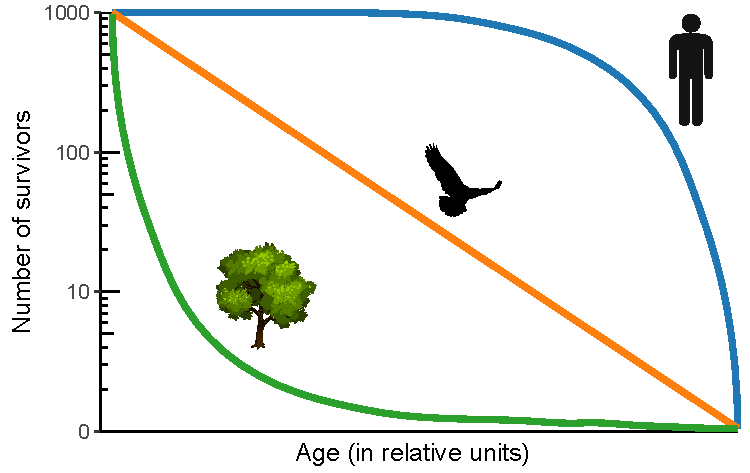
\includegraphics{chapter_materials/population_ecology/base_plot.pdf}
\caption{\label{fig:survivor-fig}Idealized examples of Types I, II, and III
survivorship curves overlaid with example organisms. Type I survivorship
is characterized by high probability of survival early in life, followed
by a rapid decline as individuals reach older age. Type II survivorship
displays roughly constant mortality throughout the lifespan of the
organism, and Type III exhibits high mortality among young offspring.}
\end{figure}

\section{Objectives}\label{objectives}

You will use the cemetery data, as well as data generated by the U.S.
Fish \& Wildlife Service \citep{milsap_bald_2016}, to address hypotheses
about different populations. We can use birth and death years on
gravestones, as well as names (to infer gender), to collect simple but
useful information to collect demographic data for the local human
population. The survivorship curve you will generate from this data will
inform some ideas about the life history strategy of humans.

Additionally, survey data collected by state and federal agencies
provide valuable information about natural population. We can use
ancillary data about individuals within a population to examine how
different forces influence demographics within a population. Golden
Eagles are federally protected in the United States, and Fish \&
Wildlife collects detailed information from tagged individuals (Fig.
\ref{fig:eagle-fig}).

\begin{figure}
\centering
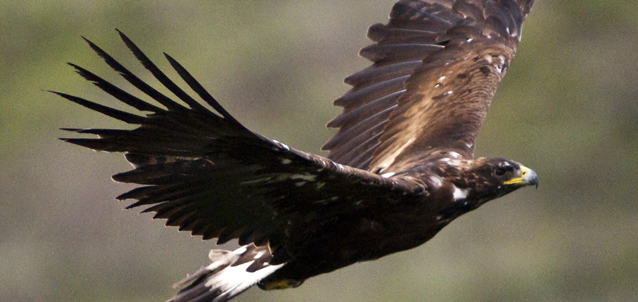
\includegraphics{chapter_materials/population_ecology/golden_eagle.jpg}
\caption{\label{fig:eagle-fig}Migratory Golden eagle in Denali National Park
and Preserve. Mating pairs return each year to northern nesting
territory in the spring, and most new fledglings leave the nest by
mid-August. During winter their range extends from southern Canada to
south of the Rocky Mountains\citep{brown_patterns_2017}.}
\end{figure}

We will use this data to test hypotheses addressing the following
questions:

\begin{enumerate}
\def\labelenumi{\arabic{enumi}.}
\tightlist
\item
  Do humans and eagles display different life history strategies?
\item
  Does gender affect survivorship in human populations?

  \begin{itemize}
  \tightlist
  \item
    And if so, how?
  \end{itemize}
\item
  Does human impact affect survivorship in eagle populations?

  \begin{itemize}
  \tightlist
  \item
    And if so, how?
  \end{itemize}
\end{enumerate}

Please form testable null hypotheses to address question number 1 and
\textbf{either} question 2 or 3 (pick one). If you want, you may also
substitute question 2 or 3 to address a hypothesis using the extra data
we generated from the gravestones (height of gravestones as a proxy of
material wealth).

To evaluate your hypotheses, you will\ldots{}

\begin{enumerate}
\def\labelenumi{\arabic{enumi}.}
\tightlist
\item
  Statistically address differences in survivorship between groups using
  a \textbf{t-test}, and display that information using a
  \textbf{bar-graph}
\item
  Unpack question 1 by \textbf{computing} and \textbf{displaying
  survivorship} (no statistical test needed for this part).
\end{enumerate}

\section{Data analysis}\label{data-analysis}

\begin{enumerate}
\def\labelenumi{\arabic{enumi}.}
\tightlist
\item
  Calculate the age at death of every individuals in both data sets
\item
  If necessary, use Excel to sort (Google it) the data based on your
  column of interest (i.e.~gender).

  \begin{itemize}
  \tightlist
  \item
    Sorting the data easily splits the population into groups that you
    can then run the calculations (below) on. If you are doing the
    entire population, you will not need to split the population, but
    for within-population questions this step will come in handy. Keep
    in mind that every time you split the data based on a categorical
    variable, you will normalize to a hypothetical population of 1000
    for the survivorship plots below.
  \end{itemize}
\item
  Calculate mean age at death, as well as a measure of variation around
  that mean for use in the \textbf{bar-graphs}.

  \begin{itemize}
  \tightlist
  \item
    The \textbf{bar-graph} is just a visual representation of the data.
    You will perform a \textbf{t-test} on this data and report the
    results to determine if the population means are actually different.
  \end{itemize}
\item
  Create a survivorship table

  \begin{itemize}
  \tightlist
  \item
    Create ``bins'' of individuals

    \begin{itemize}
    \tightlist
    \item
      0 to 1, 1 to 2, 2 to 3, etc\ldots{} for Golden Eagles
    \item
      0-9, 10-19, 20-29, etc\ldots{} for humans
    \end{itemize}
  \item
    Calculate the number of individuals surviving to that age class (the
    `countif' function in Excel will come in handy here). Keep in mind
    that for the first group you will want to count \textbf{all} of the
    observations in the data set, so your condition will be
    `\textgreater{}=0'.
  \item
    Normalize survivors to a hypothetical population of 1000

    \begin{itemize}
    \tightlist
    \item
      This will make comparisons possible between unequal sample -- so
      if you have 1250 observations in the data set, your normalized
      number for the first age class will be 1250/1250 = 1.0, which is a
      proportion you can multiply by 1000. For the second age class (if
      you have some mortality), it might be 975/1250 = 0.78, which you
      can then multiply by 1000 which equals 780.
    \end{itemize}
  \end{itemize}
\item
  Plot the number of survivors (y-axis values) against age class (x-axis
  values) to construct the survivorship curves. You may plot the data
  from the survivorship table either as normalized survivors, or on a
  logarithmic x-axis (typically how this data is displayed, as in Fig.
  \ref{fig:survivor-fig}).
\end{enumerate}

The procedure above will ultimately yield survivorship (number of
surviving individuals at a particular age class), which you may plot to
visually explore differences between groups of interest to you.

\pagebreak

\section{Lab Report Specifics}\label{lab-report-specifics}

Below are some specific guidelines for this lab report, but you should
also utilize the general grading rubric in the Syllabus!

\begin{itemize}
\item
  \textbf{Participation} (1 pts)
\item
  \textbf{Introduction} (3 pts)

  \begin{itemize}
  \tightlist
  \item
    General information about population ecology / life history
    strategies
  \item
    How are survivorship curves used in population ecology?
  \item
    Build up rationale to lead into your objectives/hypotheses
    statements.
  \end{itemize}
\item
  \textbf{Methods} (3 pts)

  \begin{itemize}
  \tightlist
  \item
    Explanation of data collection and analysis
  \end{itemize}
\item
  \textbf{Results} (6 pts)

  \begin{itemize}
  \tightlist
  \item
    Summary statistics in the text
  \item
    Bar-plots and associated t-tests for each question
  \item
    Survivorship curves for each question
  \end{itemize}
\item
  \textbf{Discussion} (3 pts)

  \begin{itemize}
  \tightlist
  \item
    Explain your results in light of your hypotheses
  \item
    What are some plausible explanations for differences (or lack
    thereof) between groups?
  \item
    Place your results in an evolutionary context.
  \end{itemize}
\end{itemize}

\chapter{Physiological Ecology}\label{physiological-ecology}

\section{Background information}\label{background-information-1}

\newcommand{\textunderscript}[1]{$_{\text{#1}}$}

In the presence of light, photosynthetic organisms can utilize light and
carbon dioxide (CO\textsubscript{2}) to make sugars - the process of
photosynthesis. The sugars made are used by these organisms (and
organisms that eat them) as a source of energy. A by-product of the
photosynthetic process is the liberation of oxygen (O\textsubscript{2}).

At the same time, these organisms are consuming oxygen via respiration.
Although respiration and photosynthesis both take place in the light, in
the dark only respiration occurs (since photosynthesis is a
light-dependent process). Though it is impossible to directly measure
gross photosynthesis (or the total amount of O\textsubscript{2} produced
\citep{wohlfahrt_many_2015}, we \emph{can} measure respiration (R) as
the \textbf{rate of O\textsubscript{2} decrease} in the dark, and the
\textbf{rate of oxygen increase} in the presence of light as a measure
of net photosynthesis (P\textsubscript{net}). Combining these direct
measurements, we can estimate gross photosynthesis
(P\textsubscript{gross}).

\begin{equation}
\color{blue} P_{net} \color{black}= \color{red}P_{gross} \color{black}- \color{blue}R
\label{eq:photosynthesis}
\end{equation}

Using equation \eqref{eq:photosynthesis}, we can use the direclty measured
terms in \color{blue} blue \color{black}, and may use them to calculate
\color{red} P\textsubscript{gross} \color{black}.

Organisms capable of photosynthesis span an incredible range of
phylogeny, from \emph{unicellular algae} to \emph{vascular plants} (Fig.
\ref{fig:organisms}). While every algae cell is photosynthetic,
\emph{aquatic macrophytes} (i.e.~vascular plants adapted to live in
aquatic ecosystems) have large amounts of specialized tissue devoted to
the transportation of resources and structural support. These two
organisms are in competition for very similar resources (such as
sunlight and dissolved nutrients) - how do their morphological
adaptations convey a competitive advantage?

\begin{figure}
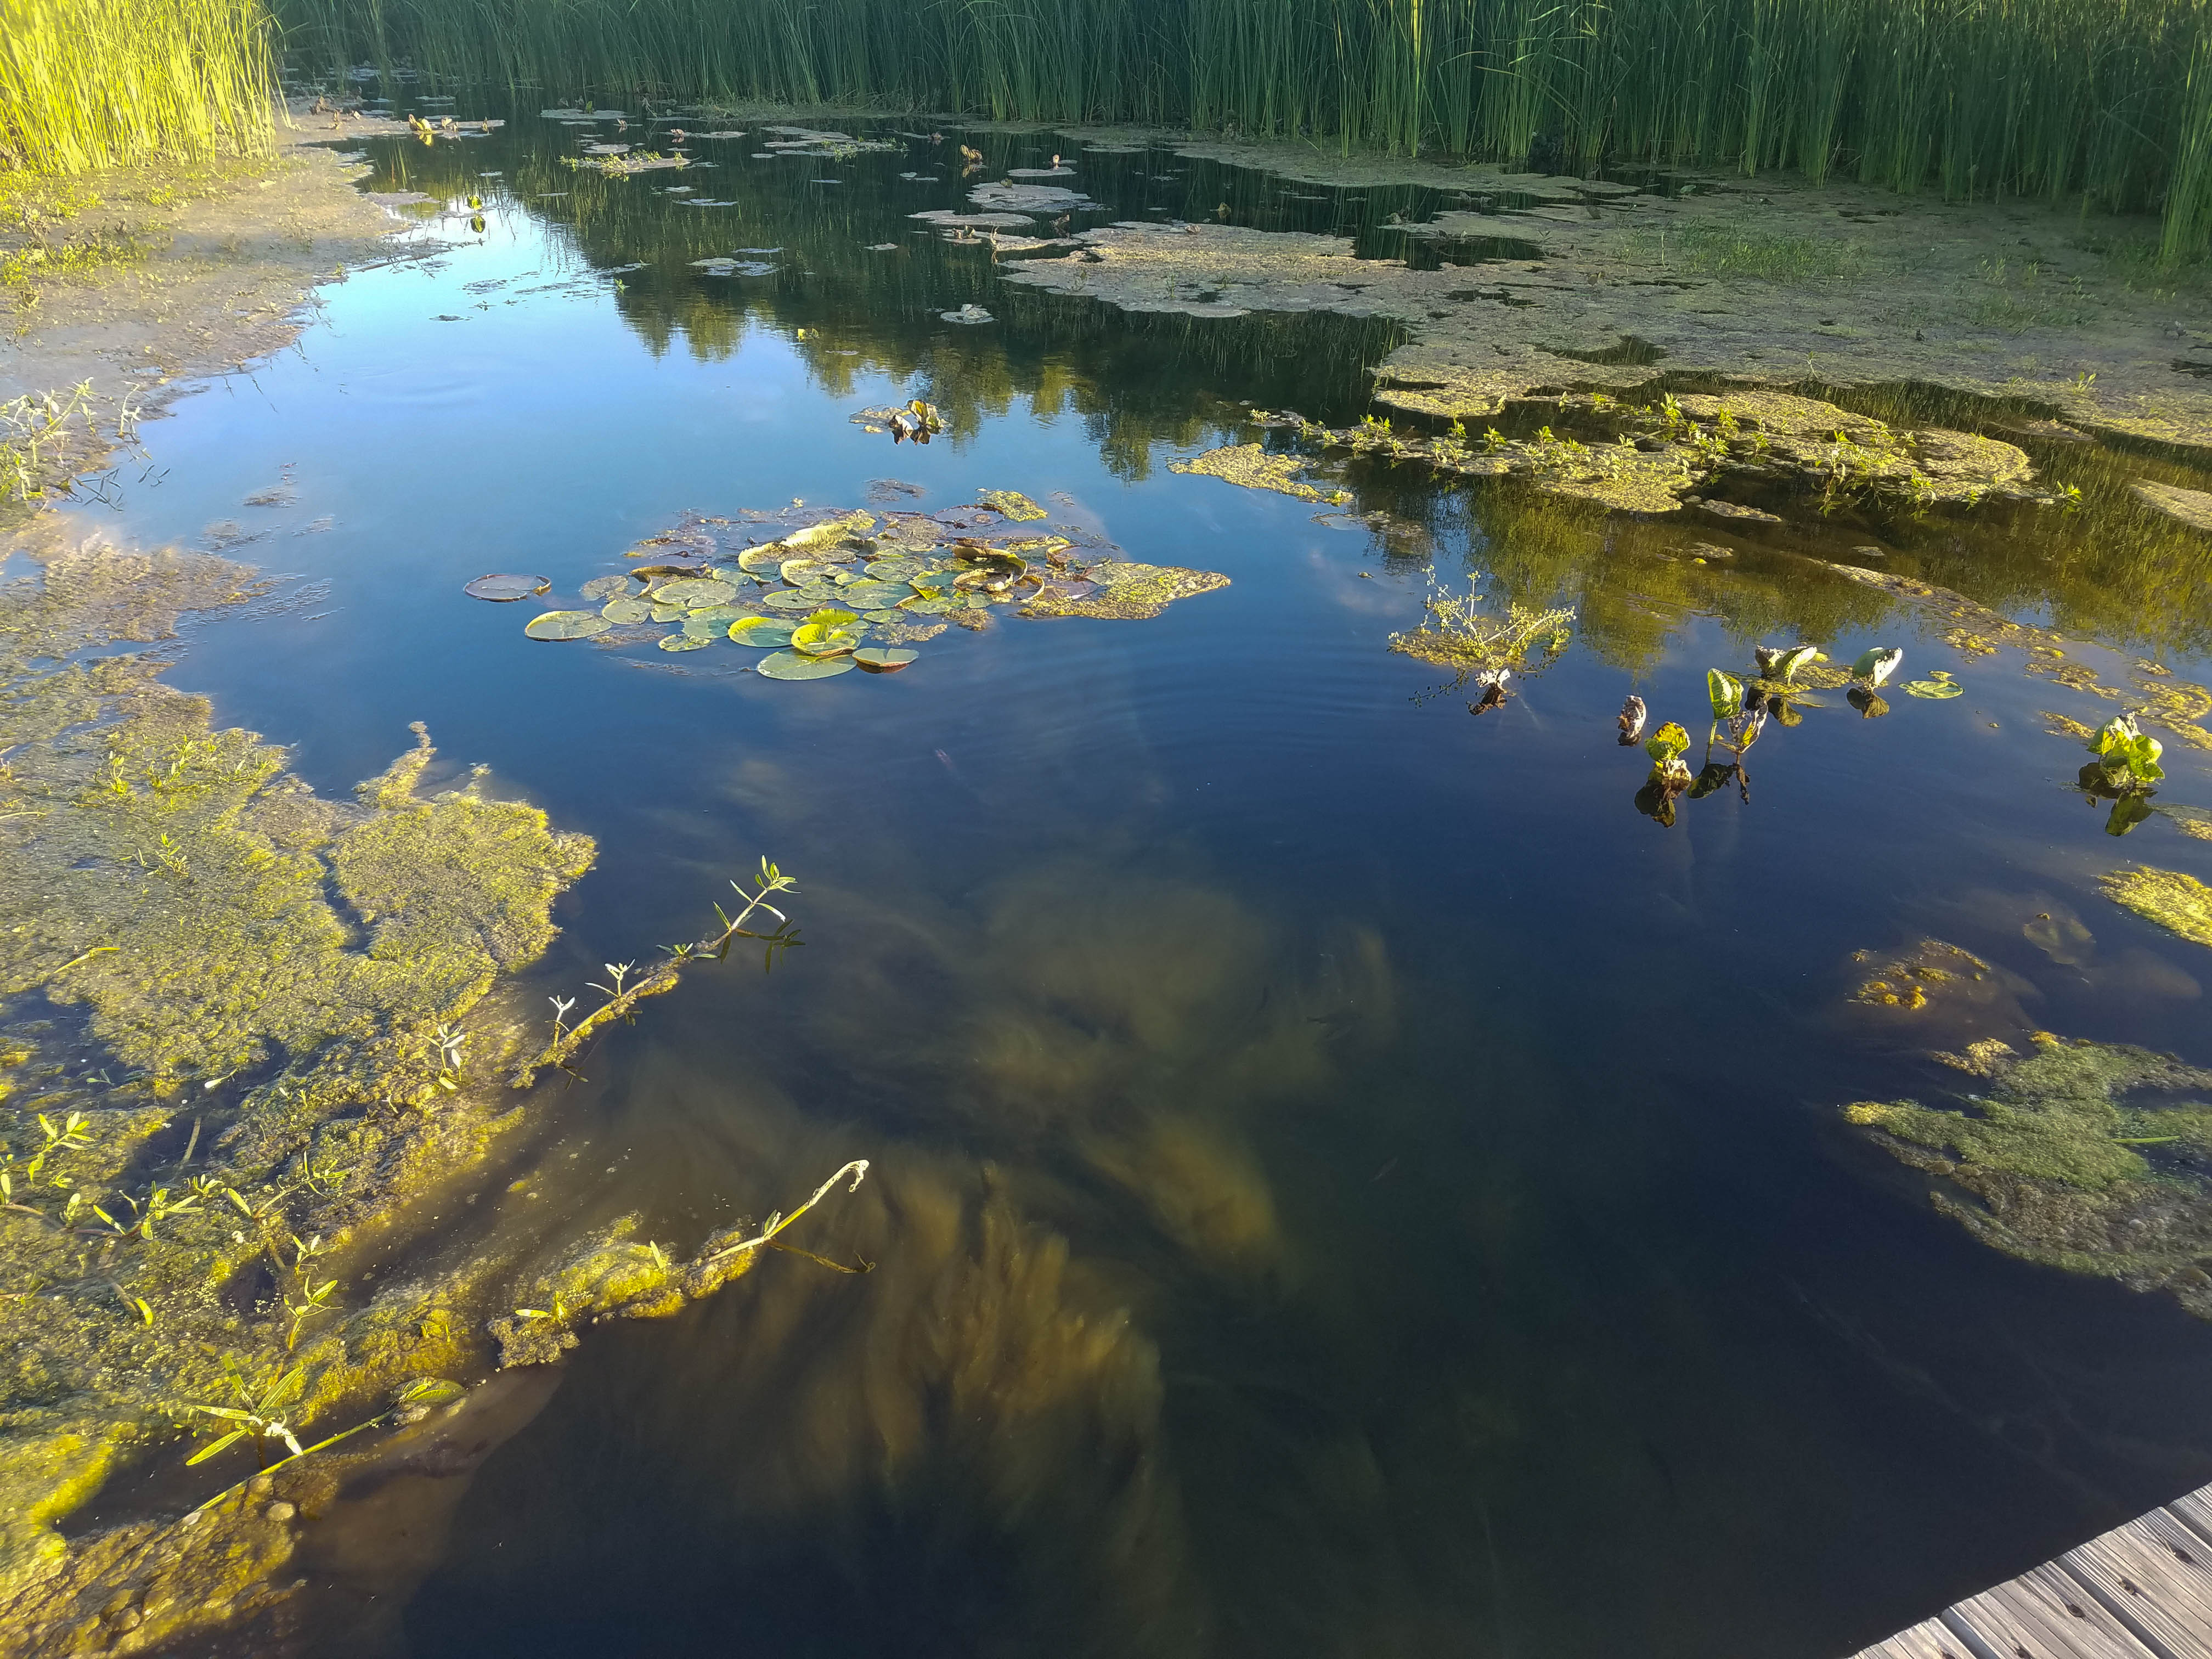
\includegraphics[width=0.5\linewidth]{chapter_materials/physiological_ecology/aquatic_photosynthesis} \includegraphics[width=0.5\linewidth]{chapter_materials/physiological_ecology/ludwigia} \caption{Aquatic algae (left pane, in both meta- and periphyton communities) and aquatic macrophytes (right pane) are photosynthetic organisms that evolved in aquatic ecosystems.}\label{fig:organisms}
\end{figure}

\section{Objectives}\label{objectives-1}

You will form hypotheses to test questions about photosynthesis in 2
aquatic organisms - algae and a common aquatic macrophyte.

\begin{enumerate}
\def\labelenumi{\arabic{enumi}.}
\item
  Which organism has the highest rate of \emph{biomass specific} gross
  photosynthesis?
\item
  Which organism has the highest rate of \emph{biomass-specific}
  respiration?
\item
  Which organism has the highest rate of net primary production (NPP)
  per day?
\end{enumerate}

\section{Materials \& methods}\label{materials-methods}

You will be using a common \textbf{oxygen-change method} to determine
rates of photosynthesis and respiration. Biological oxygen demand (BOD)
bottles use a stopper that prevents gas exchange, which provides a means
of isolating processes happening inside the bottle from the outside
environment.

\pagebreak

\subsection{Materials}\label{materials}

\begin{multicols}{2}
\begin{itemize}{}
  \item 10 L photosynthesis solution\footnote{10 L DI Water, 917 mg CaCl\textunderscript{2}, 960 mg MgSO\textunderscript{4}, 584 mg NaHCO\textunderscript{3}, 154 mg KHCO\textunderscript{3}}\\(40\% air saturation\footnote{Aerate with N\textunderscript{2} gas for 10 minutes})
  \item Samples of algae and macrophytes
  \item 330 mL BOD bottles
  \item Dissolved O\textsubscript{2} meter (DO Meter)
  \item Light source (> 400 \textmu E m\textsuperscript{-2}s\textsuperscript{-1})
  \item Aluminum foil
  \item Stir bars / stir plate
  \item Sieves (fine mesh)
  \item Forceps
  \item Drying boats (aluminum)
  \item Analytical balance \\(capable of 0.001 g)
  \item Drying oven
\end{itemize}
\end{multicols}

Oxygen production varies with the intensity of light, but reaches
saturation as light intensity increases (Fig.
\ref{fig:light-response-fig}). Since different organisms display
different light-response curves, we need to saturate their photosystems
with high light levels to account for a potential confounding variable
in our experiment.

\begin{figure}
\centering
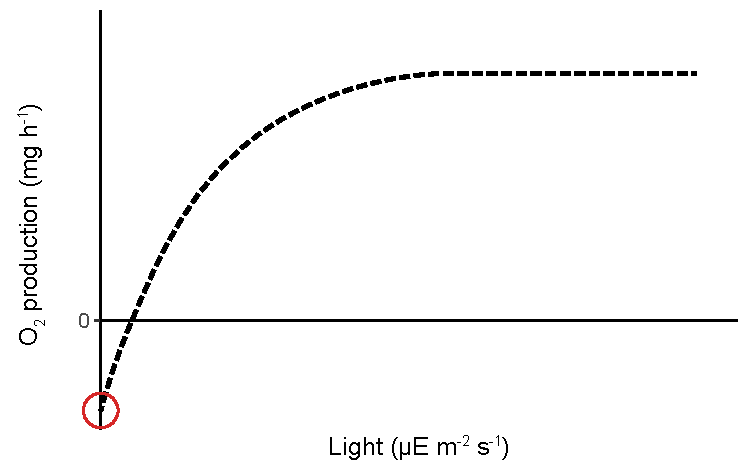
\includegraphics{chapter_materials/physiological_ecology/light_response_curve.pdf}
\caption{\label{fig:light-response-fig}A photosynthesis light-response curve
illustrates that as light intensity increases, dissolved oxygen (DO)
production eventually becomes saturated. In the dark, photosynthesis
shuts off, and respiration causes the rate of DO production to fall
below 0 (red circle on the y-axis).}
\end{figure}

\subsection{Methods}\label{methods}

\begin{enumerate}
\def\labelenumi{\arabic{enumi}.}
\tightlist
\item
  Each group will be responsible for \textbf{one} of the two species.
  Fill 9 BOD bottles with photosynthesis solution (fill to brim - the
  idea with BOD bottles is for the glass stopper to push any excess
  water out of the seal the stopper creates).
\item
  Carefully transfer a representative sample of your organism into 8 of
  the BOD bottles. Add a small stir bar to each bottle, and place the
  glass stopper and plastic cap on the bottle to seal. Use the DO probe
  to measure oxygen concentration in the remaining bottle (your control
  bottle).
\item
  You will have 4 replicates for the dark treatment, and 4 for the
  light. Wrap the dark treatment bottles in aluminum foil, and place the
  light treatment bottles under the light source.
  \underline{Record the intial times for these samples}.
\item
  While you wait (at least 1.5 hours)\ldots{}

  \begin{itemize}
  \tightlist
  \item
    Observe samples of these organisms under a dissecting/compound
    microscope and note differences in morphology. Note differences in
    the proportion of support tissues (i.e.~stems) vs.~photosynthetic
    tissues for each organism.
  \end{itemize}
\item
  After at least 1.5 hours, measure DO concentrations in the light
  bottles. Make sure to record the end time each time you take a DO
  measurement.
\item
  After 2 hours, measure the DO concentrations in the dark bottles. Make
  sure to record the end time each time you take a DO measurement.
\item
  Carefully empty the BOD bottle into a fine-mesh sieve to separate the
  sample from the photosynthesis solution. Collect/scrape the sample
  into a labeled aluminum drying tin, and place tins into a drying oven
  for 24 hrs at 105\textdegree{}C.
\end{enumerate}

\section{Data analysis}\label{data-analysis-1}

You can directly determine P\textsubscript{net} (from the light
treatment bottles) and R (from the dark treatment bottles) by
calculating the change (\textDelta) in dissolved oxygen (DO)
concentrations:

\begin{equation}
\Delta{}DO = DO_{final} - DO_{initial}
\label{eq:delta}
\end{equation}

You also recorded the elapsed incubation time(\textDelta{}h), the volume
of the BOD bottles (0.330 L), and the mass of the sample (in dry weight,
g). Using equation \eqref{eq:photosynthesis}, after getting \textDelta{}DO
normalized to volume (L) and dry weight (g), you can then calculate
P\textsubscript{gross}, or the total oxygen produced by photosynthesis
per unit biomass.

For the 1\textsuperscript{st}, and 2\textsuperscript{nd} questions, a
two-sample t-test comparing the rates of each process
(P\textsubscript{gross} and R) will tell you if there are significant
differences between each organism. Bar-graphs (with error-bars display
the stardard error of the mean) are a good way of displaying this data
visually.

The 3\textsuperscript{rd} question requires you to construct a simple
\textbf{model}. A model is a way to represent a natural process using
mathematics. Some models are simple (like the one you will construct),
and some are incredibly complex. What assumptions can you make to tackle
question 3? If we assume that these organisms respire for 24 hours a
day, and only photosynthesize when the sun is out (10 hours a day), we
can use these values as a foundation for our model (Fig.
\ref{fig:photo-model}). While this makes the maths significantly easier,
what are the limitations of this assumption?

\begin{figure}
\centering
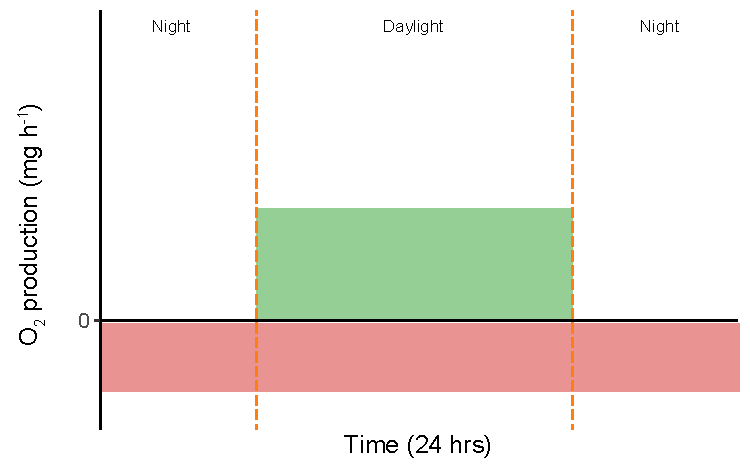
\includegraphics{chapter_materials/physiological_ecology/photo_model.pdf}
\caption{\label{fig:photo-model}A photosynthesis light-response curve
illustrates that as light intensity increases, dissolved oxygen (DO)
production eventually becomes saturated. In the dark, photosynthesis
shuts off, and respiration causes the rate of DO production to fall
below 0 (red circle on the y-axis).}
\end{figure}

There are no associated statistical tests for question 3, since you
should calculate daily values using mean P\textsubscript{gross} and mean
R (no replicate values for this question). You can present the results
of your model in the text of your results section.

\pagebreak

\section{Lab report specifics}\label{lab-report-specifics-1}

\begin{enumerate}
\def\labelenumi{\arabic{enumi}.}
\tightlist
\item
  Introduction

  \begin{itemize}
  \tightlist
  \item
    Importance of photosynthesis
  \item
    Morphological adaptations of aquatic photosynthesizers
  \item
    Objectives
  \item
    Hypotheses
  \end{itemize}
\item
  Methods

  \begin{itemize}
  \tightlist
  \item
    Oxygen change method (light/dark treatments)
  \item
    Experimental design
  \item
    Calculations / statistics / model explanation
  \end{itemize}
\item
  Results

  \begin{itemize}
  \tightlist
  \item
    Graphs/statistics for questions 1 and 2
  \item
    Results for question 3
  \end{itemize}
\item
  Discussion

  \begin{itemize}
  \tightlist
  \item
    Hypotheses rejected/supported
  \item
    Provide a coherent explanation for the patterns you see in the
    photosynthesis and respiration data (use your observations of
    morphology)
  \end{itemize}
\end{enumerate}

\pagebreak

\begin{landscape}\begin{table}[H]
\centering\begingroup\fontsize{8}{10}\selectfont
\rowcolors{2}{gray!6}{white}

\resizebox{\linewidth}{!}{
\begin{tabular}{>{\raggedright\arraybackslash}p{1cm}ll>{\raggedright\arraybackslash}p{1cm}>{\raggedright\arraybackslash}p{1cm}>{\raggedright\arraybackslash}p{1cm}>{\raggedright\arraybackslash}p{1cm}>{\raggedright\arraybackslash}p{1cm}>{\raggedright\arraybackslash}p{1cm}}
\hiderowcolors
\toprule
BOD No. & Organism & Treatment & Initial time & Initial DO (mg/L) & Final time & Final DO (mg/L) & Dish ID & Weight (g)\\
\midrule
\showrowcolors
 & Algae & Light &  &  &  &  &  & \\
 & Algae & Light &  &  &  &  &  & \\
 & Algae & Light &  &  &  &  &  & \\
 & Algae & Light &  &  &  &  &  & \\
 & Algae & Dark &  &  &  &  &  & \\
 & Algae & Dark &  &  &  &  &  & \\
 & Algae & Dark &  &  &  &  &  & \\
 & Algae & Dark &  &  &  &  &  & \\
 & Algae & Control &  &  &  &  &  & \\
 & Macrophyte & Light &  &  &  &  &  & \\
 & Macrophyte & Light &  &  &  &  &  & \\
 & Macrophyte & Light &  &  &  &  &  & \\
 & Macrophyte & Light &  &  &  &  &  & \\
 & Macrophyte & Dark &  &  &  &  &  & \\
 & Macrophyte & Dark &  &  &  &  &  & \\
 & Macrophyte & Dark &  &  &  &  &  & \\
 & Macrophyte & Dark &  &  &  &  &  & \\
 & Macrophyte & Control &  &  &  &  &  & \\
\bottomrule
\end{tabular}}
\rowcolors{2}{white}{white}\endgroup{}
\end{table}
\end{landscape}

\begin{landscape}\begin{table}[H]
\centering\begingroup\fontsize{8}{10}\selectfont
\rowcolors{2}{gray!6}{white}

\resizebox{\linewidth}{!}{
\begin{tabular}{>{\raggedright\arraybackslash}p{1cm}ll>{\raggedright\arraybackslash}p{1cm}>{\raggedright\arraybackslash}p{1cm}>{\raggedright\arraybackslash}p{1cm}>{\raggedright\arraybackslash}p{1cm}>{\raggedright\arraybackslash}p{1cm}>{\raggedright\arraybackslash}p{1cm}}
\hiderowcolors
\toprule
BOD No. & Organism & Treatment & Elapsed time (h) & Delta DO (mg/L) & Delta DO (mg) & Net Rate O2 (mg/(g*h)) & Rate (mg/(g*h)) & Daily\\
\midrule
\showrowcolors
 & Algae & Light &  &  &  &  &  & \\
 & Algae & Light &  &  &  &  &  & \\
 & Algae & Light &  &  &  &  &  & \\
 & Algae & Light &  &  &  &  &  & \\
 & Algae & Dark &  &  &  &  &  & \\
 & Algae & Dark &  &  &  &  &  & \\
 & Algae & Dark &  &  &  &  &  & \\
 & Algae & Dark &  &  &  &  &  & \\
 & Algae & Control &  &  &  &  &  & \\
 & Macrophyte & Light &  &  &  &  &  & \\
 & Macrophyte & Light &  &  &  &  &  & \\
 & Macrophyte & Light &  &  &  &  &  & \\
 & Macrophyte & Light &  &  &  &  &  & \\
 & Macrophyte & Dark &  &  &  &  &  & \\
 & Macrophyte & Dark &  &  &  &  &  & \\
 & Macrophyte & Dark &  &  &  &  &  & \\
 & Macrophyte & Dark &  &  &  &  &  & \\
 & Macrophyte & Control &  &  &  &  &  & \\
\bottomrule
\end{tabular}}
\rowcolors{2}{white}{white}\endgroup{}
\end{table}
\end{landscape}

\chapter{Biodiversity \& ecosystem
management}\label{biodiversity-ecosystem-management}

\section{Background information}\label{background-information-2}

Community ecology depends directly on our ability to quantify the
various species that compose the community or a component of the
community (such as the plants present). Quantification of community
composition is essential for understanding changes through time or
impacts of management actions. This week we will quantify the community
composition of wetland plants at the Lake Waco Wetlands (LWWs).

The LWWs has historically been strongly dominated by \emph{Typha}
(cattail). Although native to Texas, cattails are very agressive and
frequently dominant wetlands to the exclusion of other species. To
counter this dominance tendency, managers have tried to increase the
diversity of the plant community in some areas of the LWWs by planting
other species {[}especially \emph{Schenoplectus} (bulrush) and
\emph{Pontederia} (pickerelweed){]}, or by hand-harvesting cattail out
of some areas in the hopes that other species will colonize the open
areas (Fig. \ref{fig:restoration-fig}).

\begin{figure}
\centering
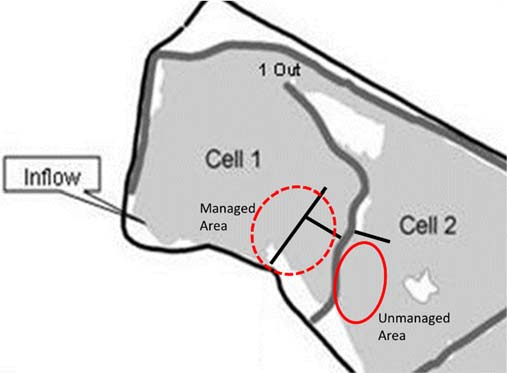
\includegraphics{chapter_materials/restoration_ecology/lww_management.jpg}
\caption{\label{fig:restoration-fig}Map showing cells 1 and 2 of the Lake
Waco Wetlands (LWWs). The boardwalk in cell 1 has had frequent
management for several years (dotted red circle), while cell 2 has had
no mmanagement (solid red circle).}
\end{figure}

\section{Objectives}\label{objectives-2}

You will collect vegetation data from two zones in the LWWs which have
different management histories. One area in Cell 1 adjacent to the
floating boardwalk is a high visitation area where frequent management
has taken place. In contrast, Cell 2 has had virtually no management.
Five transects will be made originating from the boardwalk (cell 1) and
from the levee (cell 2). Data about community composition will be
recorded from 5 quadrats (area of 1 m\textsuperscript{2}) along each
transect.

\pagebreak
Using the data generated and appropriate statistical analyses
(contingency table or t-test), address the following questions:

\begin{enumerate}
\def\labelenumi{\arabic{enumi}.}
\tightlist
\item
  Is management activity influencing the \textbf{abundance} of cattail?

  \begin{itemize}
  \tightlist
  \item
    A 2x2 contingency table is appropriate for this question.
  \end{itemize}
\item
  Is management activity influencing the \textbf{dominance} of cattail?

  \begin{itemize}
  \tightlist
  \item
    A 2x2 contingency table is appropriate for this question.
  \end{itemize}
\item
  Is management activity influencing \textbf{species richness}?

  \begin{itemize}
  \tightlist
  \item
    Could be addressed using a 2x2 contingency table or a t-test.
  \end{itemize}
\item
  Does cattail dominance influence \textbf{species richness}?

  \begin{itemize}
  \tightlist
  \item
    Could be addressed using a 2x2 contingency table or a t-test. For
    this question, the grouping variable is \emph{cattail dominance}, so
    you should use data from both cells!
  \end{itemize}
\end{enumerate}

\pagebreak

\section{Lab report specifics}\label{lab-report-specifics-2}

\begin{enumerate}
\def\labelenumi{\arabic{enumi}.}
\tightlist
\item
  Introduction

  \begin{itemize}
  \tightlist
  \item
    Why is biodiversity important?
  \item
    Why sample vegetation?
  \item
    Objectives
  \item
    Hypotheses
  \end{itemize}
\item
  Methods

  \begin{itemize}
  \tightlist
  \item
    Experimental design
  \item
    Review how data was collected
  \item
    Calculations / statistics
  \end{itemize}
\item
  Results

  \begin{itemize}
  \tightlist
  \item
    Question 1 (text \textbf{AND} graph/table)
  \item
    Question 2 (text \textbf{AND} graph/table)
  \item
    Question 3 (text \textbf{AND} graph/table)
  \item
    Question 4 (text \textbf{AND} graph/table)
  \end{itemize}
\item
  Discussion

  \begin{itemize}
  \tightlist
  \item
    Hypotheses rejected/supported
  \item
    Provide a coherent explanation/interpretation of your results
  \end{itemize}
\end{enumerate}

\bibliography{book.bib,packages.bib}

\backmatter
\printindex

\end{document}
